\documentclass{article}

\usepackage[margin=1in]{geometry}
\usepackage{listings}
\usepackage{color}
\usepackage{graphicx}
\usepackage{float}

\definecolor{dkgreen}{rgb}{0,0.6,0}
\definecolor{gray}{rgb}{0.5,0.5,0.5}
\definecolor{mauve}{rgb}{0.58,0,0.82}

\lstset{frame=tb,
	language=C,
	aboveskip=3mm,
	belowskip=3mm,
	showstringspaces=false,
	columns=flexible,
	basicstyle={\small\ttfamily},
	numbers=left,
	numberstyle=\color{gray},
	keywordstyle=\color{blue},
	commentstyle=\color{dkgreen},
	stringstyle=\color{mauve},
	breaklines=true,
	breakatwhitespace=true,
	tabsize=4
}

\title{Final Project: Bluetooth Controlled Car}
\date{December 15, 2017}
\author{Matthew Friedman 861151348\\Souradeep Bhattacharya 861105938\\EE128 Section: 021}
\begin{document}
	\maketitle
	\section*{Project Description}
	\subsection*{Summary}
	\par Our objective was to design and build a remote controlled car that could be controlled with a smartphone or any other Bluetooth enabled master device.
	\subsection*{Requirements/Goals}
	The car must be able to:
	\begin{itemize}
		\item The car must be able to move in 4 standard directions
		\subitem Forward
		\subitem Backward
		\subitem Left
		\subitem Right
		\item The car must abe able to move in the 4 combination directions
		\subitem Forward-Left
		\subitem Forward-Right
		\subitem Backward-Left
		\subitem Backward-Right
		\item The car must be able to turn on and off headlights
		\item The car must be able to turn on and off a horn
		\item The car must be able to drive as straight as possible with out the use of external sensors.
		\item The car's control circuitry must be made as simply as possible with no extraneous parts.
	\end{itemize}
	\section*{System Design}
	\subsection*{Block Diagram}
	\begin{figure}[H]
		\centering
		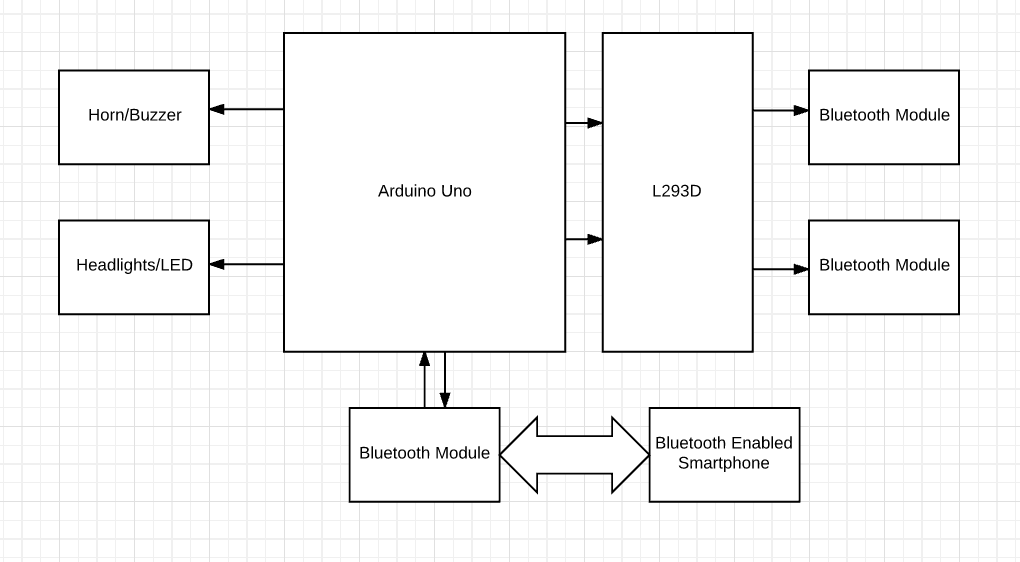
\includegraphics[scale=0.70]{BD}
		\caption{Overall System Block Diagram}
	\end{figure}
	\subsection*{Flow Charts}
	\begin{figure}[H]
		\centering
		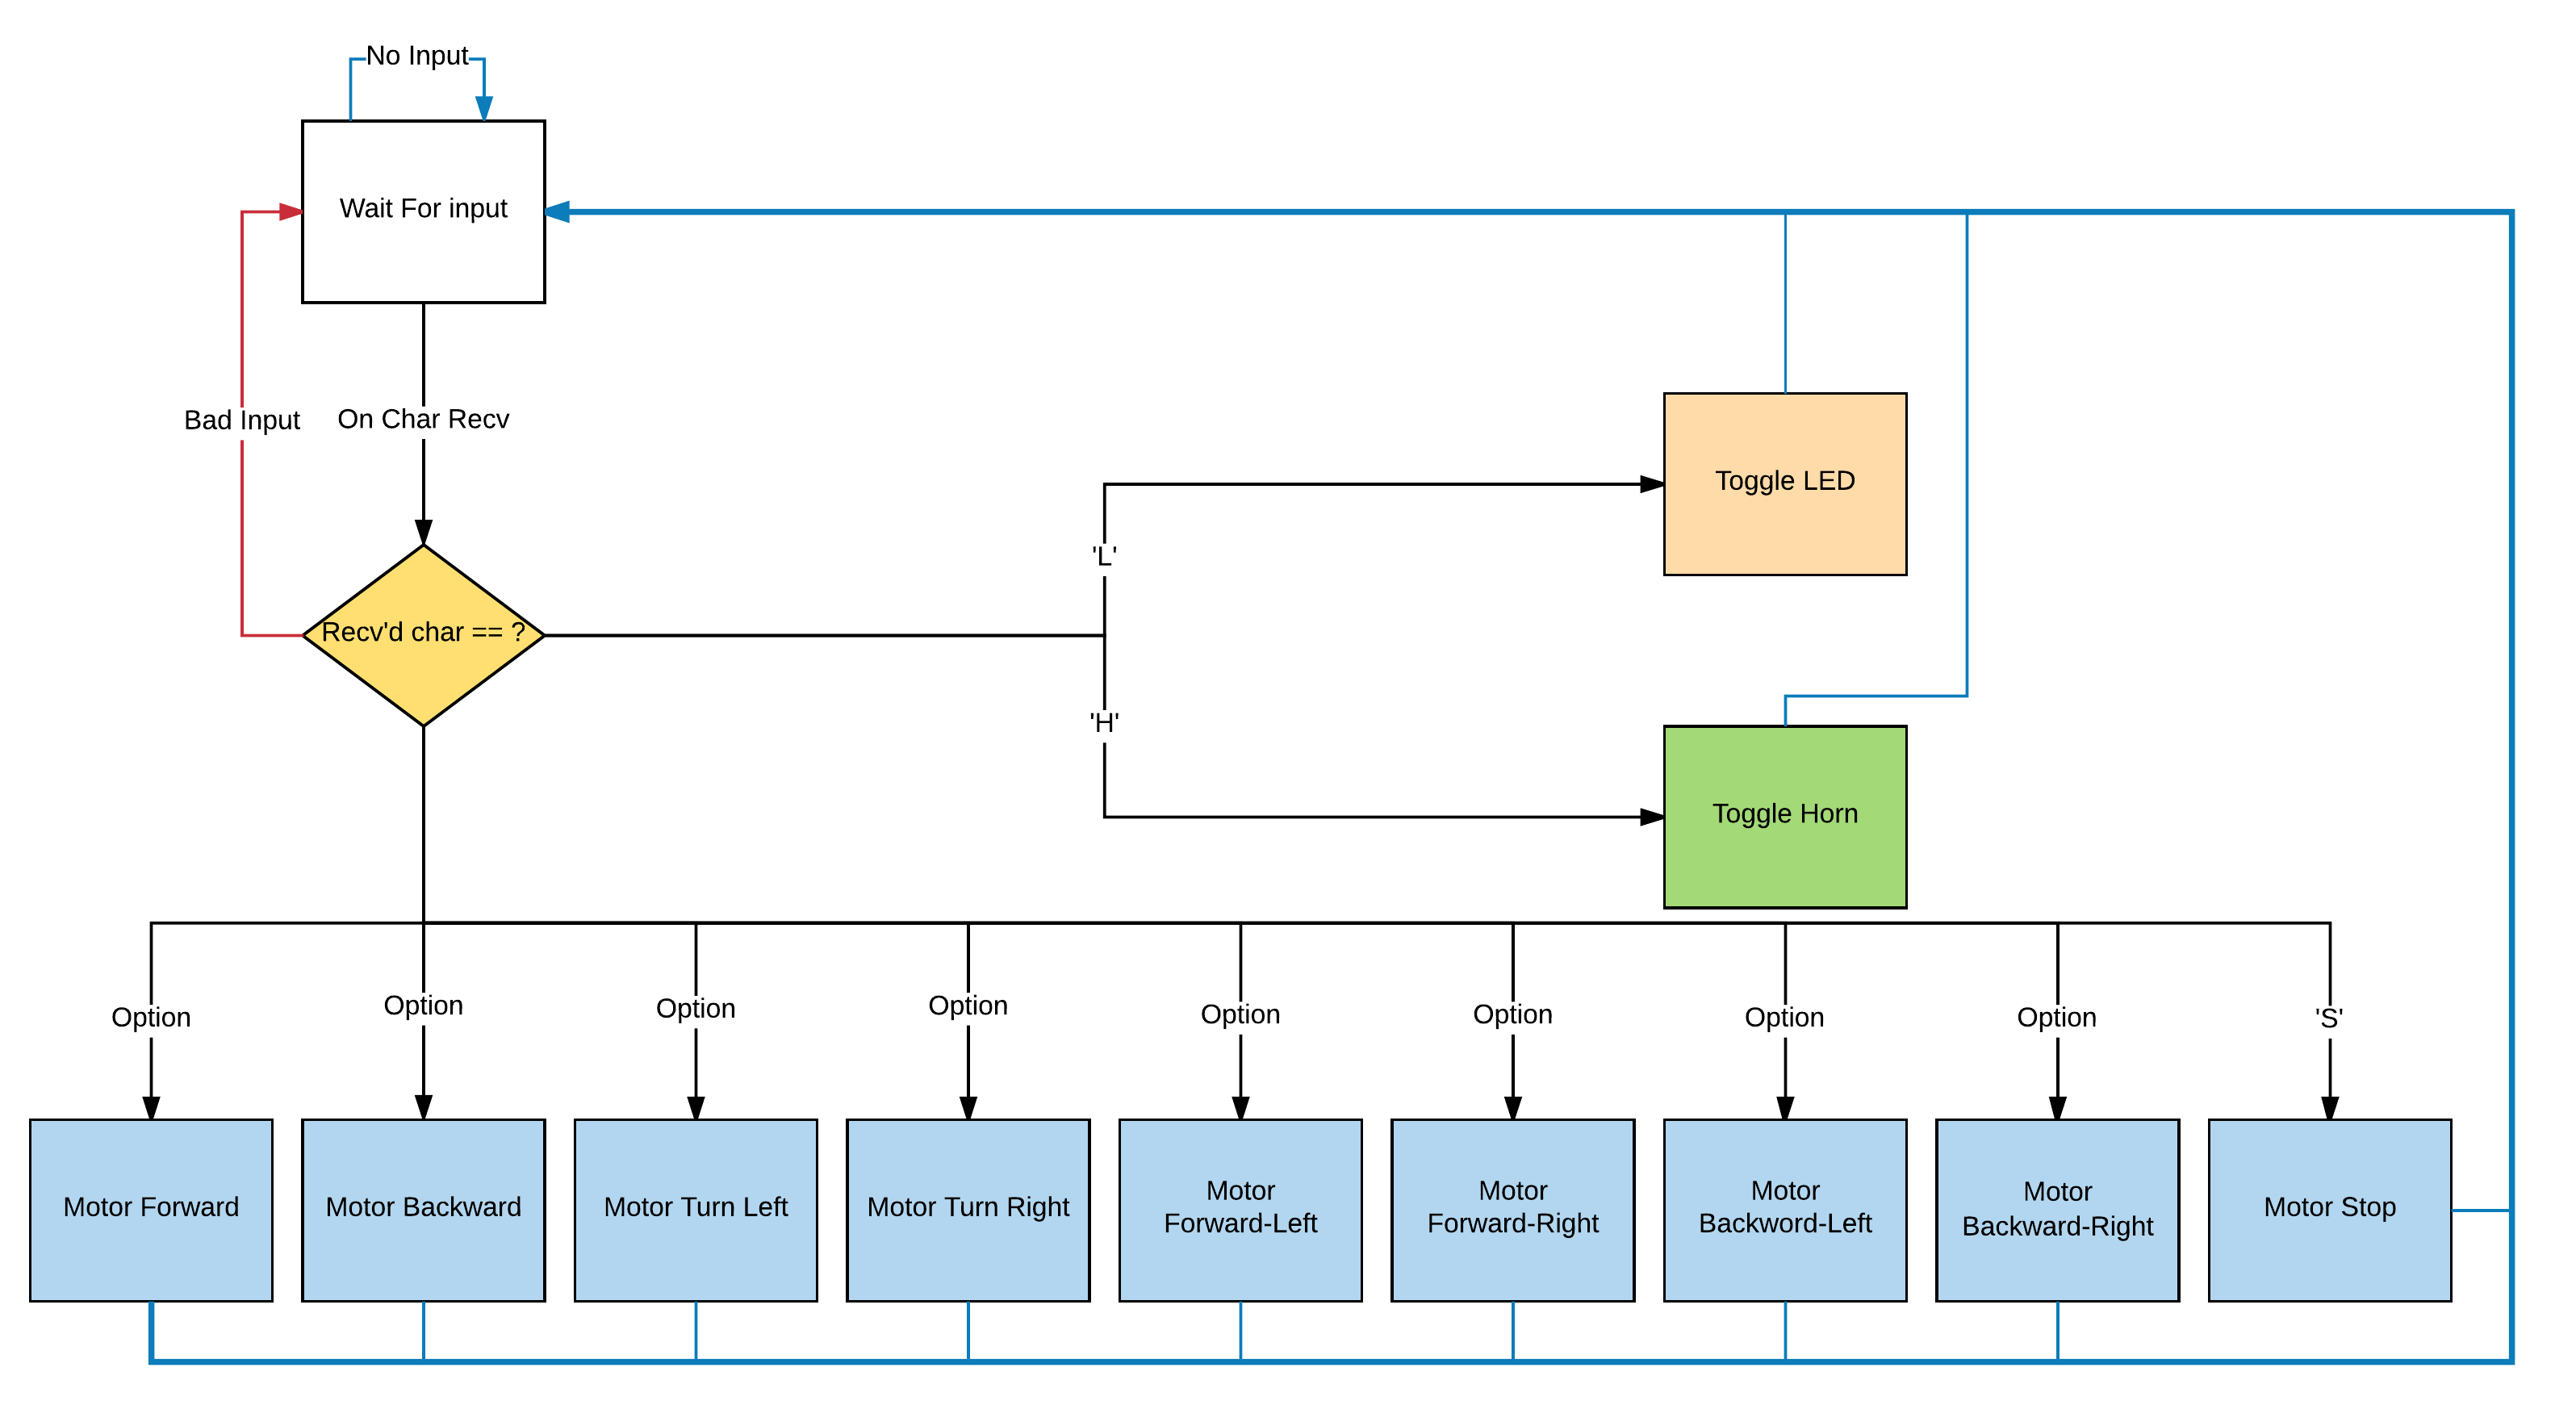
\includegraphics[scale=0.15]{FD}
		\caption{Overall System Block Diagram}
	\end{figure}
	\section*{Implementation Details}
	\subsection*{Schematic}
	\subsubsection*{Overall}
	\begin{figure}[H]
		\centering
		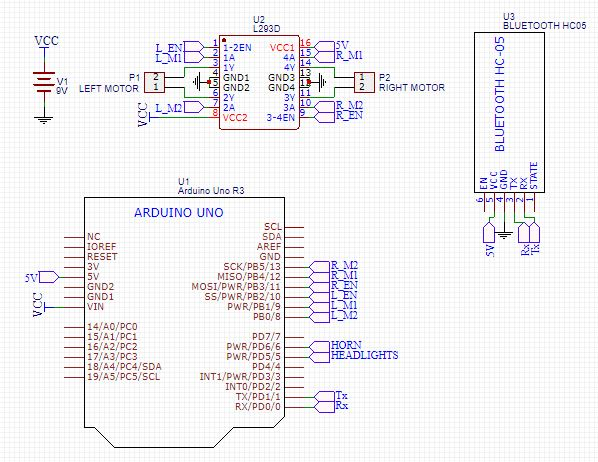
\includegraphics[scale=1.0]{overview}
		\caption{Overall System Schematic}
	\end{figure}
	\subsubsection*{Detailed Portions of Schematic}
	
	\begin{figure}[H]
		\centering
		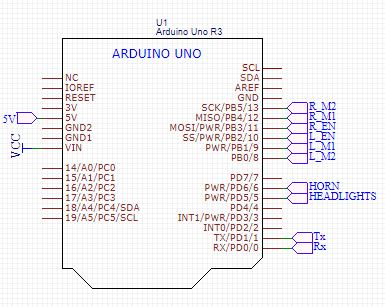
\includegraphics[scale=1.0]{uno}
		\caption{Close up of the Arduino Uno}
	\end{figure}
	
	\begin{figure}[H]
		\centering
		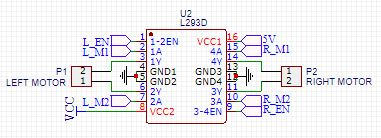
\includegraphics[scale=1.0]{l293d}
		\caption{Close up of the Motor driver}
	\end{figure}
	
	\subsection*{Key Code Portion}
	\subsubsection*{Main Loop}
	\begin{lstlisting}
	void loop() 
	{
		//check for bt val
		if(Serial.available())
		{
			bt_char = Serial.read();
			Serial.println(bt_char);
			Serial.flush();
		}
		
		// Conduct action based on BT Value
		switch(bt_char)
		{
			case LIGHT_CHAR:
				toggle_headlights();
			break;
			
			case HORN_CHAR:
				toggle_horn();
			break;
			
			case FOR_CHAR:
				set_motor(FOR);
			break;
			
			case BACK_CHAR:
				set_motor(BACK);
			break;
			
			case CCW_CHAR:
				set_motor(CCW);
			break;
			
			case CW_CHAR:
				set_motor(CW);
			break;
			
			case STOP_CHAR:
				set_motor(STOP);
			break;
			
			case FW_LEFT:
				set_motor(FL);
			break;
			
			case FW_RIGHT:
				set_motor(FR);
			break;
			
			case BACK_LEFT:
				set_motor(BL);
			break;
			
			case BACK_RIGHT:
				set_motor(BR);
			break;
			
			default:
				set_motor(STOP);
			break;
		}
		delay(5); //200 ticks per second
	}
		
	\end{lstlisting}
	
	\subsubsection*{Motor control}
	\begin{lstlisting}
	void set_motor(int dir)
	{
		switch(dir)
		{
			case STOP:
				//stop
				//Serial.println("Stop");
				analogWrite(L_EN, BASE_SPEED + L_M_OFFSET);
				analogWrite(R_EN, BASE_SPEED);
				digitalWrite(L_M1, LOW);
				digitalWrite(L_M2, LOW);
				digitalWrite(R_M1, LOW);
				digitalWrite(R_M2, LOW);
			break;
			
			case BACK:
				//backward
				//Serial.println("Back");
				analogWrite(L_EN, BASE_SPEED + L_M_OFFSET);
				analogWrite(R_EN, BASE_SPEED);
				digitalWrite(L_M1, HIGH);
				digitalWrite(L_M2, LOW);
				digitalWrite(R_M1, HIGH);
				digitalWrite(R_M2, LOW);
			break;
			
			case FOR:
				//forward
				//Serial.println("Forward");
				analogWrite(L_EN, BASE_SPEED + L_M_OFFSET);
				analogWrite(R_EN, BASE_SPEED);
				digitalWrite(L_M1, LOW);
				digitalWrite(L_M2, HIGH);
				digitalWrite(R_M1, LOW);
				digitalWrite(R_M2, HIGH);
			break;
			
			case CW:
				//rotate CW
				//Serial.println("CCW");
				analogWrite(L_EN, BASE_SPEED + L_M_OFFSET);
				analogWrite(R_EN, BASE_SPEED);
				digitalWrite(L_M1, HIGH);
				digitalWrite(L_M2, LOW);
				digitalWrite(R_M1, LOW);
				digitalWrite(R_M2, HIGH);
			break;
			
			case CCW:
				//rotate CCW
				//Serial.println("CW");
				analogWrite(L_EN, BASE_SPEED + L_M_OFFSET);
				analogWrite(R_EN, BASE_SPEED);
				digitalWrite(L_M1, LOW);
				digitalWrite(L_M2, HIGH);
				digitalWrite(R_M1, HIGH);
				digitalWrite(R_M2, LOW);
			break;
			
			case FL:
				// Forwards Left
				analogWrite(L_EN, BASE_SPEED + L_M_OFFSET);
				analogWrite(R_EN, BASE_SPEED + DIAG_OFFSET);
				digitalWrite(L_M1, LOW);
				digitalWrite(L_M2, HIGH);
				digitalWrite(R_M1, LOW);
				digitalWrite(R_M2, HIGH);
			break;
			
			case FR:
				// Fowards Right
				analogWrite(L_EN, BASE_SPEED + L_M_OFFSET + DIAG_OFFSET);
				analogWrite(R_EN, BASE_SPEED);
				digitalWrite(L_M1, LOW);
				digitalWrite(L_M2, HIGH);
				digitalWrite(R_M1, LOW);
				digitalWrite(R_M2, HIGH);
			break;
			
			case BL:
				// Backwards Left
				analogWrite(L_EN, BASE_SPEED + L_M_OFFSET);
				analogWrite(R_EN, BASE_SPEED + DIAG_OFFSET);
				digitalWrite(L_M1, HIGH);
				digitalWrite(L_M2, LOW);
				digitalWrite(R_M1, HIGH);
				digitalWrite(R_M2, LOW);
			break;
			
			case BR:
				// Backwards Right
				analogWrite(L_EN, BASE_SPEED + L_M_OFFSET + DIAG_OFFSET);
				analogWrite(R_EN, BASE_SPEED);
				digitalWrite(L_M1, HIGH);
				digitalWrite(L_M2, LOW);
				digitalWrite(R_M1, HIGH);
				digitalWrite(R_M2, LOW);
			break;
			
			default:
				//stop
				//Serial.println("Stop");
				digitalWrite(L_M1, LOW);
				digitalWrite(L_M2, LOW);
				digitalWrite(R_M1, LOW);
				digitalWrite(R_M2, LOW);
			break;
		}
	}
	\end{lstlisting}
	
	\section*{Testing/Evaluation}
	\par 
	We tested the car by driving it around in lab mostly. We were able to use the lines in between tiles to see how straight the car was going. We then adjusted the value and tried again. We also drove the car around in lab to test the maximum range of the Bluetooth.
	\section*{Discussions}
	\subsection*{Challenges}
	One of the challenges was find a Bluetooth App that would work right out of the box on our phones. We found an app that simply transmits a character on a press or release of a button.
	\subsection*{Limitations}
	One of our motors was weaker then the other and resulted in the car wanting to turn to the left. In order to correct for this we had a small offset value for that motor that we added whenever we did an analogue write. This required us to calibrate the value whenever changes were made to the car, like tightening the wheel.
	\subsection*{Possible Improvements}
	Adding an external sensor, like a pair of rotary encoders, may result in a much better ability for the car to drive straight. We could have fed back the sensor value to the MCU and used a PID control system to adjust the car to keep it going straight. We could have also written a simple Bluetooth app using MIT App Inventor to also send the offset value for the motors and have the user calibrate the system.
	\section*{Roles and Responsibilities}
	\paragraph{Matthew} Designed Car and built car. Wrote primary code, primary calibration, assisted on report.
	\paragraph{Gogol} Wrote code to allow for combination movement, some calibration in lab, wrote report and documentation.
	\section*{Conclusion}
	In this project we created a Bluetooth Remote Controlled Car. We didn't have any major difficulties implementing this project. We did have to adjust for the fact that one of the motors was stronger than the other, but that was easily adjusted by controlling the PWM for the enable.
	
	\pagebreak
	\section*{Appendix}
	\subsection*{Code}
	\begin{lstlisting}
	//define pins
	#define L_EN 10
	#define R_EN 11
	#define L_M1 9
	#define L_M2 8
	#define R_M1 12
	#define R_M2 13
	#define HORN 6
	#define HEADLIGHT 5
	
	//directions
	#define FOR 1
	#define BACK 2
	#define CCW 3
	#define CW 4
	#define STOP 5
	#define FL 6
	#define FR 7
	#define BL 8
	#define BR 9
	
	//BT
	char bt_char = '0';
	#define FOR_CHAR 'F'
	#define BACK_CHAR 'B'
	#define CCW_CHAR 'R'
	#define CW_CHAR 'L'
	#define STOP_CHAR 'S'
	#define LIGHT_CHAR 'W'
	#define HORN_CHAR 'V'
	#define FW_LEFT 'G'
	#define FW_RIGHT 'I'
	#define BACK_LEFT 'H'
	#define BACK_RIGHT 'J'
	
	//globals
	bool horn_stat = false;
	bool light_stat = false;
	int L_M_OFFSET = 25;
	int BASE_SPEED = 150;
	int DIAG_OFFSET = 80;
	
	//function prototypes
	void set_motor(int dir);
	void toggle_horn();
	void toggle_headlights();
	
	void setup() 
	{
		//pin modes
		pinMode(HORN, OUTPUT);
		pinMode(HEADLIGHT, OUTPUT);
		pinMode(L_EN, OUTPUT);
		pinMode(R_EN, OUTPUT);
		pinMode(L_M1, OUTPUT);
		pinMode(L_M2, OUTPUT);
		pinMode(R_M1, OUTPUT);
		pinMode(R_M2, OUTPUT);
		
		//setup BT
		Serial.begin(9600);
		
		//set initial motor dir to stop and set enables
		analogWrite(L_EN, BASE_SPEED + L_M_OFFSET);
		analogWrite(R_EN, BASE_SPEED);
		set_motor(STOP);
		toggle_headlights();
	}
	
	void loop() 
	{
		//check for bt val
		if(Serial.available())
		{
			bt_char = Serial.read();
			Serial.println(bt_char);
			Serial.flush();
		}
	
		// Conduct action based on BT Value
		switch(bt_char)
		{
			case LIGHT_CHAR:
				toggle_headlights();
			break;
			
			case HORN_CHAR:
				toggle_horn();
			break;
			
			case FOR_CHAR:
				set_motor(FOR);
			break;
			
			case BACK_CHAR:
				set_motor(BACK);
			break;
			
			case CCW_CHAR:
				set_motor(CCW);
			break;
	
			case CW_CHAR:
				set_motor(CW);
			break;
	
			case STOP_CHAR:
				set_motor(STOP);
			break;
	
			case FW_LEFT:
				set_motor(FL);
			break;
	
			case FW_RIGHT:
				set_motor(FR);
			break;
	
			case BACK_LEFT:
				set_motor(BL);
			break;
			
			case BACK_RIGHT:
				set_motor(BR);
			break;
	
			default:
				set_motor(STOP);
			break;
		}
		delay(5); //200 ticks per second
	}
	
	void set_motor(int dir)
	{
		switch(dir)
		{
			case STOP:
				//stop
				//Serial.println("Stop");
				analogWrite(L_EN, BASE_SPEED + L_M_OFFSET);
				analogWrite(R_EN, BASE_SPEED);
				digitalWrite(L_M1, LOW);
				digitalWrite(L_M2, LOW);
				digitalWrite(R_M1, LOW);
				digitalWrite(R_M2, LOW);
			break;
			
			case BACK:
				//backward
				//Serial.println("Back");
				analogWrite(L_EN, BASE_SPEED + L_M_OFFSET);
				analogWrite(R_EN, BASE_SPEED);
				digitalWrite(L_M1, HIGH);
				digitalWrite(L_M2, LOW);
				digitalWrite(R_M1, HIGH);
				digitalWrite(R_M2, LOW);
			break;
			
			case FOR:
				//forward
				//Serial.println("Forward");
				analogWrite(L_EN, BASE_SPEED + L_M_OFFSET);
				analogWrite(R_EN, BASE_SPEED);
				digitalWrite(L_M1, LOW);
				digitalWrite(L_M2, HIGH);
				digitalWrite(R_M1, LOW);
				digitalWrite(R_M2, HIGH);
			break;
			
			case CW:
				//rotate CW
				//Serial.println("CCW");
				analogWrite(L_EN, BASE_SPEED + L_M_OFFSET);
				analogWrite(R_EN, BASE_SPEED);
				digitalWrite(L_M1, HIGH);
				digitalWrite(L_M2, LOW);
				digitalWrite(R_M1, LOW);
				digitalWrite(R_M2, HIGH);
			break;
			
			case CCW:
				//rotate CCW
				//Serial.println("CW");
				analogWrite(L_EN, BASE_SPEED + L_M_OFFSET);
				analogWrite(R_EN, BASE_SPEED);
				digitalWrite(L_M1, LOW);
				digitalWrite(L_M2, HIGH);
				digitalWrite(R_M1, HIGH);
				digitalWrite(R_M2, LOW);
			break;
			
			case FL:
				// Forwards Left
				analogWrite(L_EN, BASE_SPEED + L_M_OFFSET);
				analogWrite(R_EN, BASE_SPEED + DIAG_OFFSET);
				digitalWrite(L_M1, LOW);
				digitalWrite(L_M2, HIGH);
				digitalWrite(R_M1, LOW);
				digitalWrite(R_M2, HIGH);
			break;
			
			case FR:
				// Fowards Right
				analogWrite(L_EN, BASE_SPEED + L_M_OFFSET + DIAG_OFFSET);
				analogWrite(R_EN, BASE_SPEED);
				digitalWrite(L_M1, LOW);
				digitalWrite(L_M2, HIGH);
				digitalWrite(R_M1, LOW);
				digitalWrite(R_M2, HIGH);
			break;
			
			case BL:
				// Backwards Left
				analogWrite(L_EN, BASE_SPEED + L_M_OFFSET);
				analogWrite(R_EN, BASE_SPEED + DIAG_OFFSET);
				digitalWrite(L_M1, HIGH);
				digitalWrite(L_M2, LOW);
				digitalWrite(R_M1, HIGH);
				digitalWrite(R_M2, LOW);
			break;
			
			case BR:
				// Backwards Right
				analogWrite(L_EN, BASE_SPEED + L_M_OFFSET + DIAG_OFFSET);
				analogWrite(R_EN, BASE_SPEED);
				digitalWrite(L_M1, HIGH);
				digitalWrite(L_M2, LOW);
				digitalWrite(R_M1, HIGH);
				digitalWrite(R_M2, LOW);
			break;
			
			default:
				//stop
				//Serial.println("Stop");
				digitalWrite(L_M1, LOW);
				digitalWrite(L_M2, LOW);
				digitalWrite(R_M1, LOW);
				digitalWrite(R_M2, LOW);
			break;
		}
	}
	
	void toggle_horn()
	{
		//Serial.println("Horn");
		horn_stat = !(horn_stat);
		if(horn_stat)
		{
			//horn on
			analogWrite(HORN, 255/2);
		}
		else
		{
			//horn off
			digitalWrite(HORN, LOW);
		}
	}
	
	void toggle_headlights()
	{
		//Serial.println("Headlights");
		light_stat = !(light_stat);
		if(light_stat)
		{
			//light on
			digitalWrite(HEADLIGHT, HIGH);
		}
		else
		{
			//light off
			digitalWrite(HEADLIGHT, LOW);
		}
	}
	\end{lstlisting}
\end{document}